\documentclass[10pt,a4paper]{article}

\usepackage[utf8]{inputenc}

\usepackage[T1]{fontenc}

\usepackage{geometry}

\usepackage{ragged2e}

\usepackage{graphicx}

\graphicspath{{../7 Main/}}

\usepackage{booktabs}

\usepackage{amsmath}

\usepackage{array}

\usepackage{float}

\usepackage{hyperref}

\hypersetup{colorlinks=true, linkcolor=blue, urlcolor=blue, citecolor=blue, pdfborder={0 0 0}}

\geometry{margin=1.55cm}

\setlength{\parindent}{0pt}

\title{Cross-Sectional Return Prediction for Global Banks\\with Rolling Kernel Calibration}

\author{Francesco Florio \\ Pierfrancesco Meloni \\ Salvatore Messina \\ Alice Sisto \\ Martina Zavatteri}

\date{}

\begin{document}

\maketitle

\begin{abstract}

This project predicts next-day USD log returns for a global universe of 25 listed banks and converts the forecasts into constrained long-only portfolios. The information set starts from 77 daily market and macro-financial covariate series, from which 15 standardised modelling inputs are selected for the rolling prediction panel. Bank returns are computed from Yahoo adjusted close when available, so dividend and split adjustments enter the daily return ratios. The active rolling evaluation covers 2005-01-03 -- 2025-12-30 over 42 semi-annual blocks. The mandatory linear kernel is compared with degree-2 polynomial and Gaussian/RBF kernels, plus an equal-weight benchmark. Kernel portfolios are constructed only through constrained regularised mean-variance optimisation with 1\%-7\% asset bounds, training-window covariance estimates and validation-selected covariance regularisation. The rolling blocks are independent and processed in parallel with a configurable worker count. The chosen design is a roughly twenty-year active evaluation, 2005-01-01 -- 2025-12-31, after an initial calibration and validation period starting in 2003-01-01. All data outputs, figures and code are organised and explained in the GitHub repository cited in the References.

\end{abstract}

\section{Executive Checklist}

\begin{table}[H]\centering\small

\begin{tabular}{>{\raggedright\arraybackslash}p{0.35\textwidth}>{\raggedright\arraybackslash}p{0.57\textwidth}}

\toprule

Requirement & Final implementation \\

\midrule

Bank panel & Daily USD adjusted-return panel for 25 active listed banks across US, UK, EU, Switzerland and Japan. \\

Active period & Design active period 2005-01-01 -- 2025-12-31; realised common period 2005-01-03 -- 2025-12-30, with 42 rolling active blocks. \\

Dividend adjustment & Yahoo \texttt{Adj Close} is used when available; \texttt{Close} is only a fallback for missing adjusted prices. \\

No look-ahead & Signals are formed at date \(t\); targets are next-day close-to-close USD log returns. \\

Rolling calibration & 18 months train, 6 months validation, then 6 active months out of sample. \\

Initial calibration & First active block starts in 2005-01-01, using the preceding 24 months, approximately 2003-01-01 -- 2004-12-31. \\

Model inputs & 77 daily numerical covariate series in the covariate file; 15 standardised inputs used in the active model panel, plus regional information from the bank universe. \\

Models & Mandatory linear ridge benchmark, degree-2 polynomial and Gaussian/RBF specifications. \\

Portfolio construction & Constrained regularised mean-variance using kernel forecasts, training-window covariance, validation-selected \(\gamma\), and 1\%--7\% asset bounds. \\

Parallel design & 42 independent semi-annual rolling blocks; desktop runs start from 10 configurable workers and aggregate outputs by block/date order. \\

Benchmarks & Equal-weight portfolio and linear kernel portfolio. \\

Diagnostics & Cumulative return, drawdown, rolling Sharpe, crisis windows, weight dynamics, geographic exposure, forecast \(R^2\), normality tests and tail diagnostics. \\

\bottomrule

\end{tabular}

\end{table}

\section{Data and Timing}

The active universe is an empirical implementation choice. The assignment does not impose a fixed list of banks, so the code keeps listed institutions with usable Yahoo price history from the start of the project sample, allowing a short grace period for local exchange holidays. This gives a tractable global bank panel, but it also creates an important caveat: selecting banks with long usable histories can introduce survivorship bias, especially in a sector where failed or delisted institutions are economically meaningful.

Prices are downloaded with yfinance automatic adjustment disabled, then the dataset notebook explicitly chooses \texttt{Adj Close} when it is present and positive. Only if the adjusted series is missing does the code fall back to \texttt{Close}. The target is therefore a dividend- and split-adjusted total-return proxy rather than a pure price return. Non-USD listings are converted into USD before log returns are computed, so forecasts and portfolio performance are measured in a common currency.

The project calendar is daily, not only trading days. If one local exchange is closed, the latest adjusted local price is carried forward and the corresponding tradable flag is false. The asset remains in the portfolio, but it cannot be actively rebalanced until the local market opens again. This is important because US, UK, euro-area, Swiss and Japanese bank holidays do not line up perfectly.

The cleaning rule separates valuation from tradability. Forward-filled prices are used to keep a continuous daily valuation panel, but the flag records whether the asset and the relevant FX rate were actually observed on that date. A return is marked usable only when both the current and previous USD observations are tradable. This avoids treating stale holiday prices as fresh market information while still allowing the portfolio value to be carried across non-trading days. The dataset notebook also writes an audit file for the active bank universe, so the common start date and excluded candidates can be checked rather than inferred from the final return matrix.

\begin{figure}[H]\centering

\includegraphics[width=0.96\textwidth]{img/asset_price_tradable_bands.png}
\caption{Normalised USD bank prices. Red shading marks dates where at least one asset is not tradable (weekends and holidays), so the panel keeps valuation continuity while preserving the trading calendar constraint.}
\end{figure}

\section{Why Banks?}

The bank universe is not only a convenient sector choice. The economic motivation is that a portfolio-weighting algorithm should ideally react to revenue drivers that can be observed at high frequency. In many industries, near-real-time revenue estimates require alternative data: store foot traffic, card spending, shipping data, web traffic, or geopolitical news. Those signals are expensive, noisy and often unavailable in a clean academic project. For banks, one core revenue channel is more directly connected to observable market prices: the spread between the rate at which banks lend and the rate at which they fund themselves.

This is why the covariate set emphasises interest rates, real rates, yield-curve information and credit spreads. These variables move more slowly than single-name equity prices on an ordinary day, but they can reprice quickly when the monetary-policy regime changes. During quantitative easing, quantitative tightening, inflation surprises or funding-stress episodes, rate and spread markets aggregate expectations about future policy, future inflation, whether inflation is anchored, and perceived credit risk. In that sense they provide a continuous market-based proxy for drivers that quarterly accounting data would reveal only with a delay.

The objective is therefore not pure momentum maximisation. The hope is that market-based covariates make the strategy more responsive during crises and policy turning points, reducing drawdowns and letting compounding work through smaller losses. Equity-index covariates are included for the same reason: they are daily proxies for national and regional growth when a continuous GDP indicator is not available. FX variables also matter because dollar strength, euro weakness or yen moves can identify risk-on/risk-off momentum and cross-border stress, especially for global banks reporting or trading across currencies.

\section{No Look-Ahead Controls}

The timing convention is close-to-next-close. On rebalance date \(t\), the model uses only information observable by the date-\(t\) close and predicts the USD log return from close \(t\) to close \(t+1\). The next-day shift appears only in the target columns, not in the covariates. Cross-sectional normalisation is computed date by date, while market-wide covariates use expanding moments through the current date.

The implementation includes the following no look-ahead controls. Future target leakage is avoided because target columns are created with a next-day shift and are excluded from the feature set. Scaling leakage is avoided because cross-sectional z-scores are computed using only observations from the current date, while time-series z-scores rely on expanding moments available up to the current date. Hyperparameter tuning is also performed without future information, since each active block uses only the preceding training and validation windows. Closed markets are handled by keeping the previous portfolio weight for the closed asset, rather than treating it as tradable. Finally, adjusted close prices are preferred, so dividend-related price drops do not contaminate capital-return targets.

\vspace{-0.75cm}

\begin{figure}[H]
\centering
\begin{minipage}{0.645\textwidth}
    \centering
    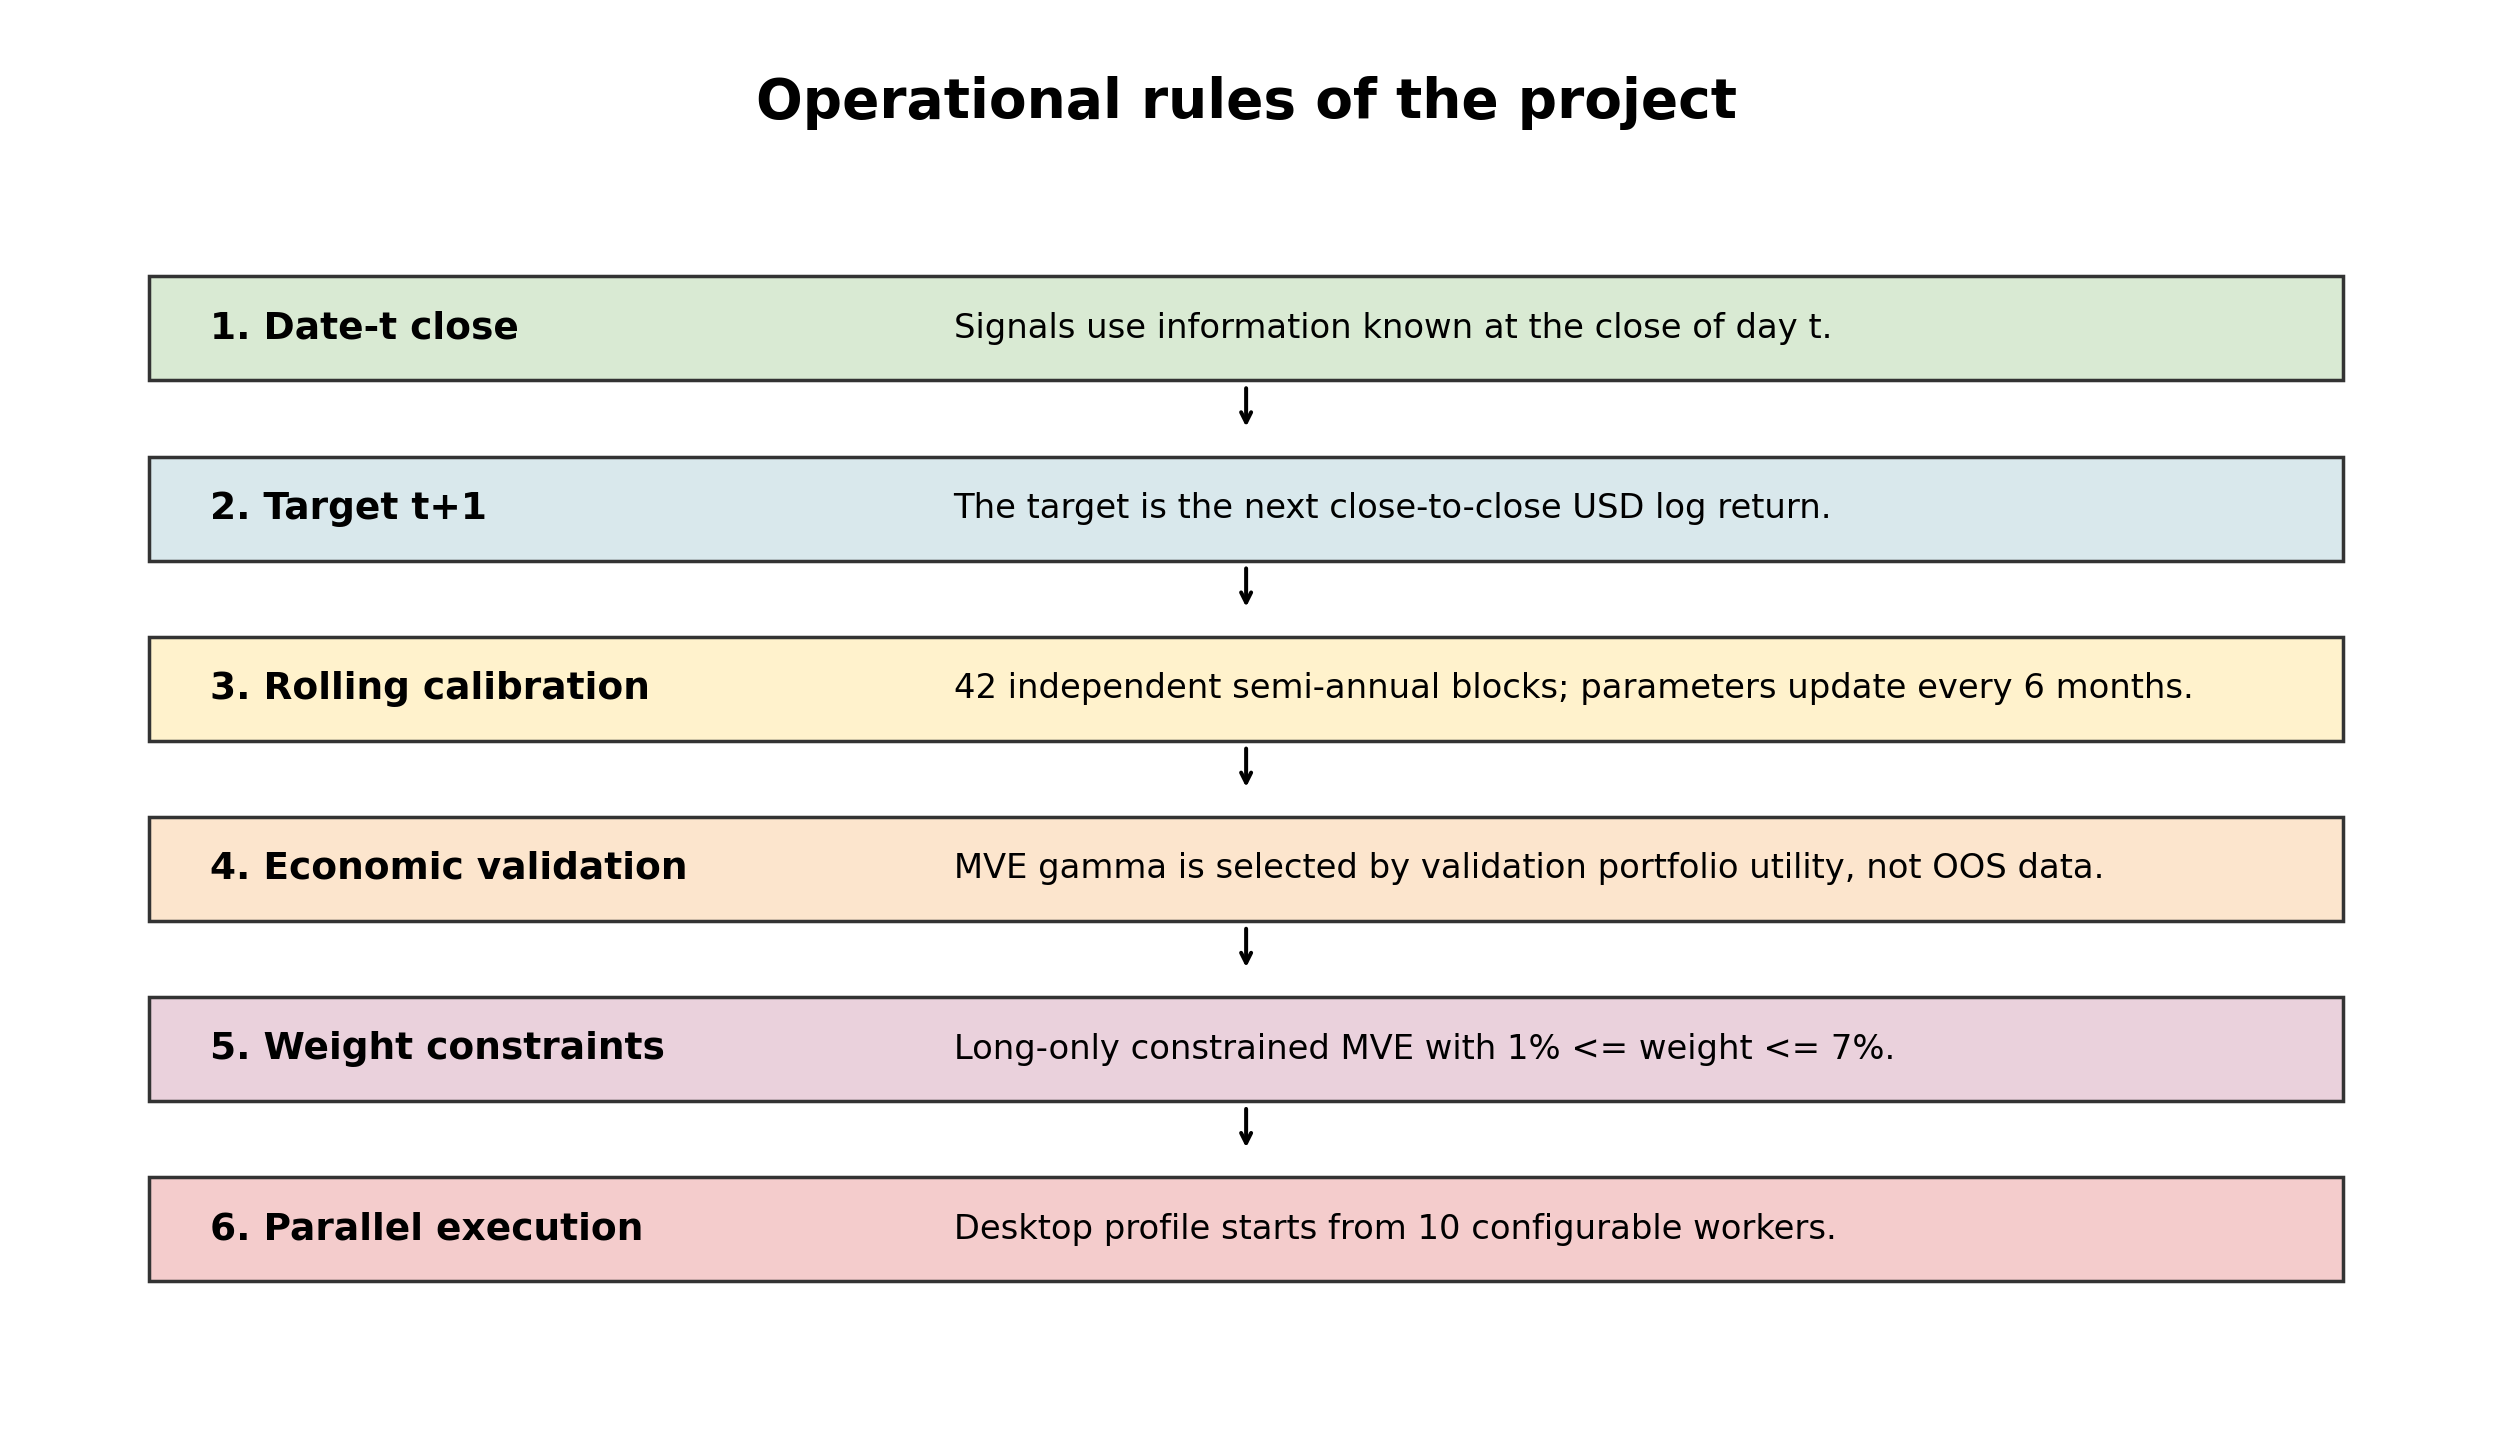
\includegraphics[width=\textwidth]{img/project_rules.png}
\end{minipage}
\hfill
\begin{minipage}{0.3\textwidth}
    \centering
    \vspace{0.5cm}
    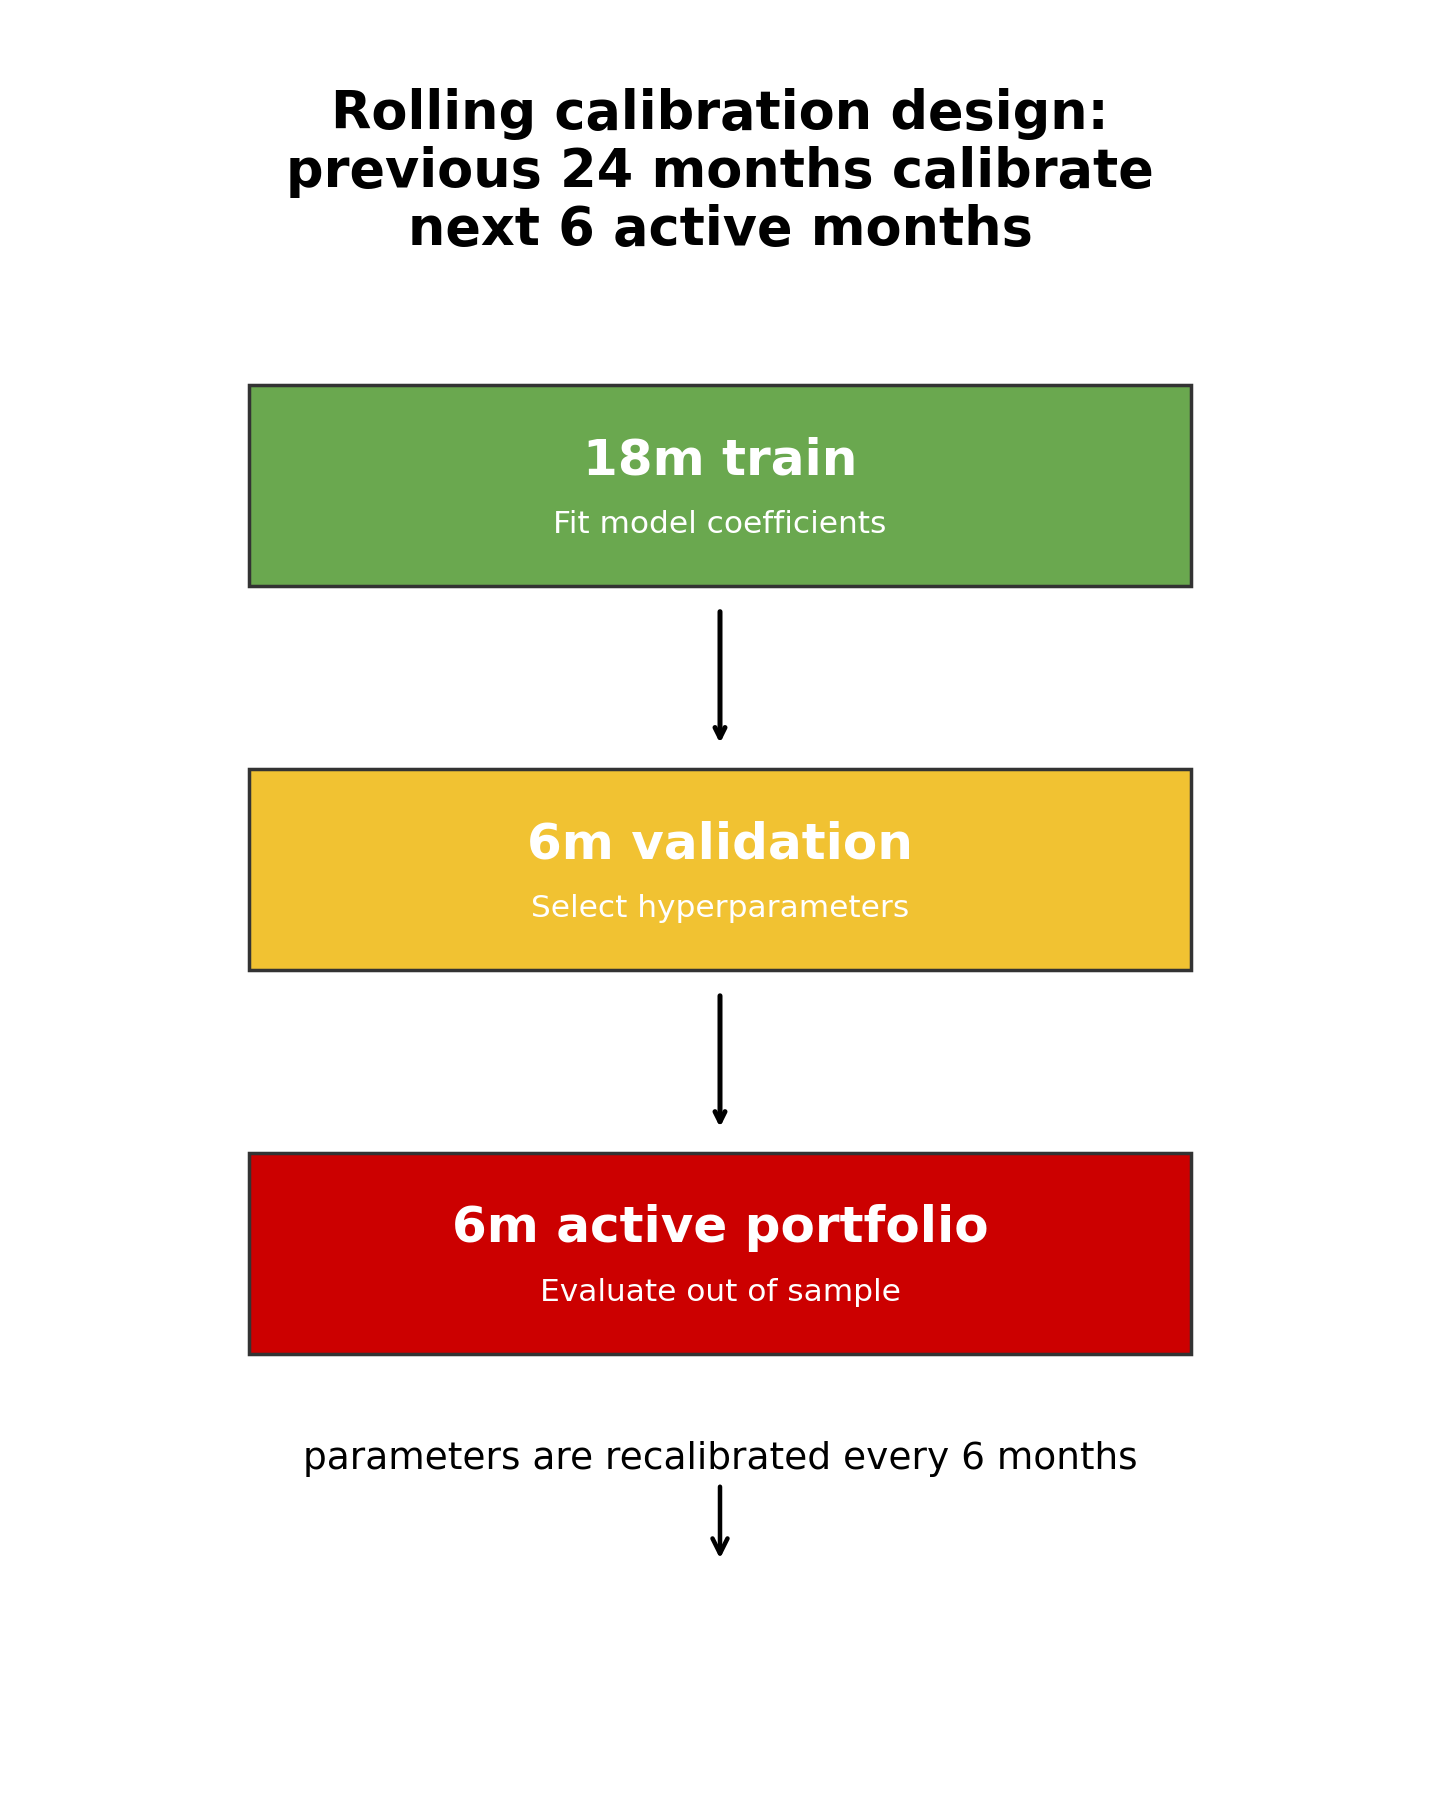
\includegraphics[width=\textwidth]{img/sample_split.png}
     \vspace{-0.15cm}
\end{minipage}

\vspace{-1cm}
\end{figure}

\section{Daily Covariates}

The covariate file contains 77 daily numerical series after raw market levels, log returns and rate changes are aligned on the project calendar. The rolling model does not feed every raw column directly into the kernel: it uses 15 standardised model inputs selected from the daily bank and macro-financial information set. Bank-specific variables include one-day USD returns, absolute return measures and relative cross-sectional movement.\\



\begin{minipage}{\textwidth}
\begin{minipage}[t]{0.28\textwidth}
\justifying
\noindent
 Common variables include VIX, regional equity-index returns, financial-sector proxies, FX moves, US Treasury yields, credit spreads and regional rate series when available.\\
 
\noindent
The objective is not to build a large accounting dataset; it is to keep the information set daily, market-based and observable at the same frequency as the target.\\

\noindent
The normalisation step is economically important. Kernel methods depend on inner products or distances between feature vectors, so a variable with a mechanically larger scale can dominate the model if it is not standardised. Bank-level variables are therefore z-scored within each date, while common time-series variables are scaled with expanding moments known at date \(t\).
\end{minipage}
\hfill
\begin{minipage}[t]{0.68\textwidth}
\centering
\vspace{-0.2cm}
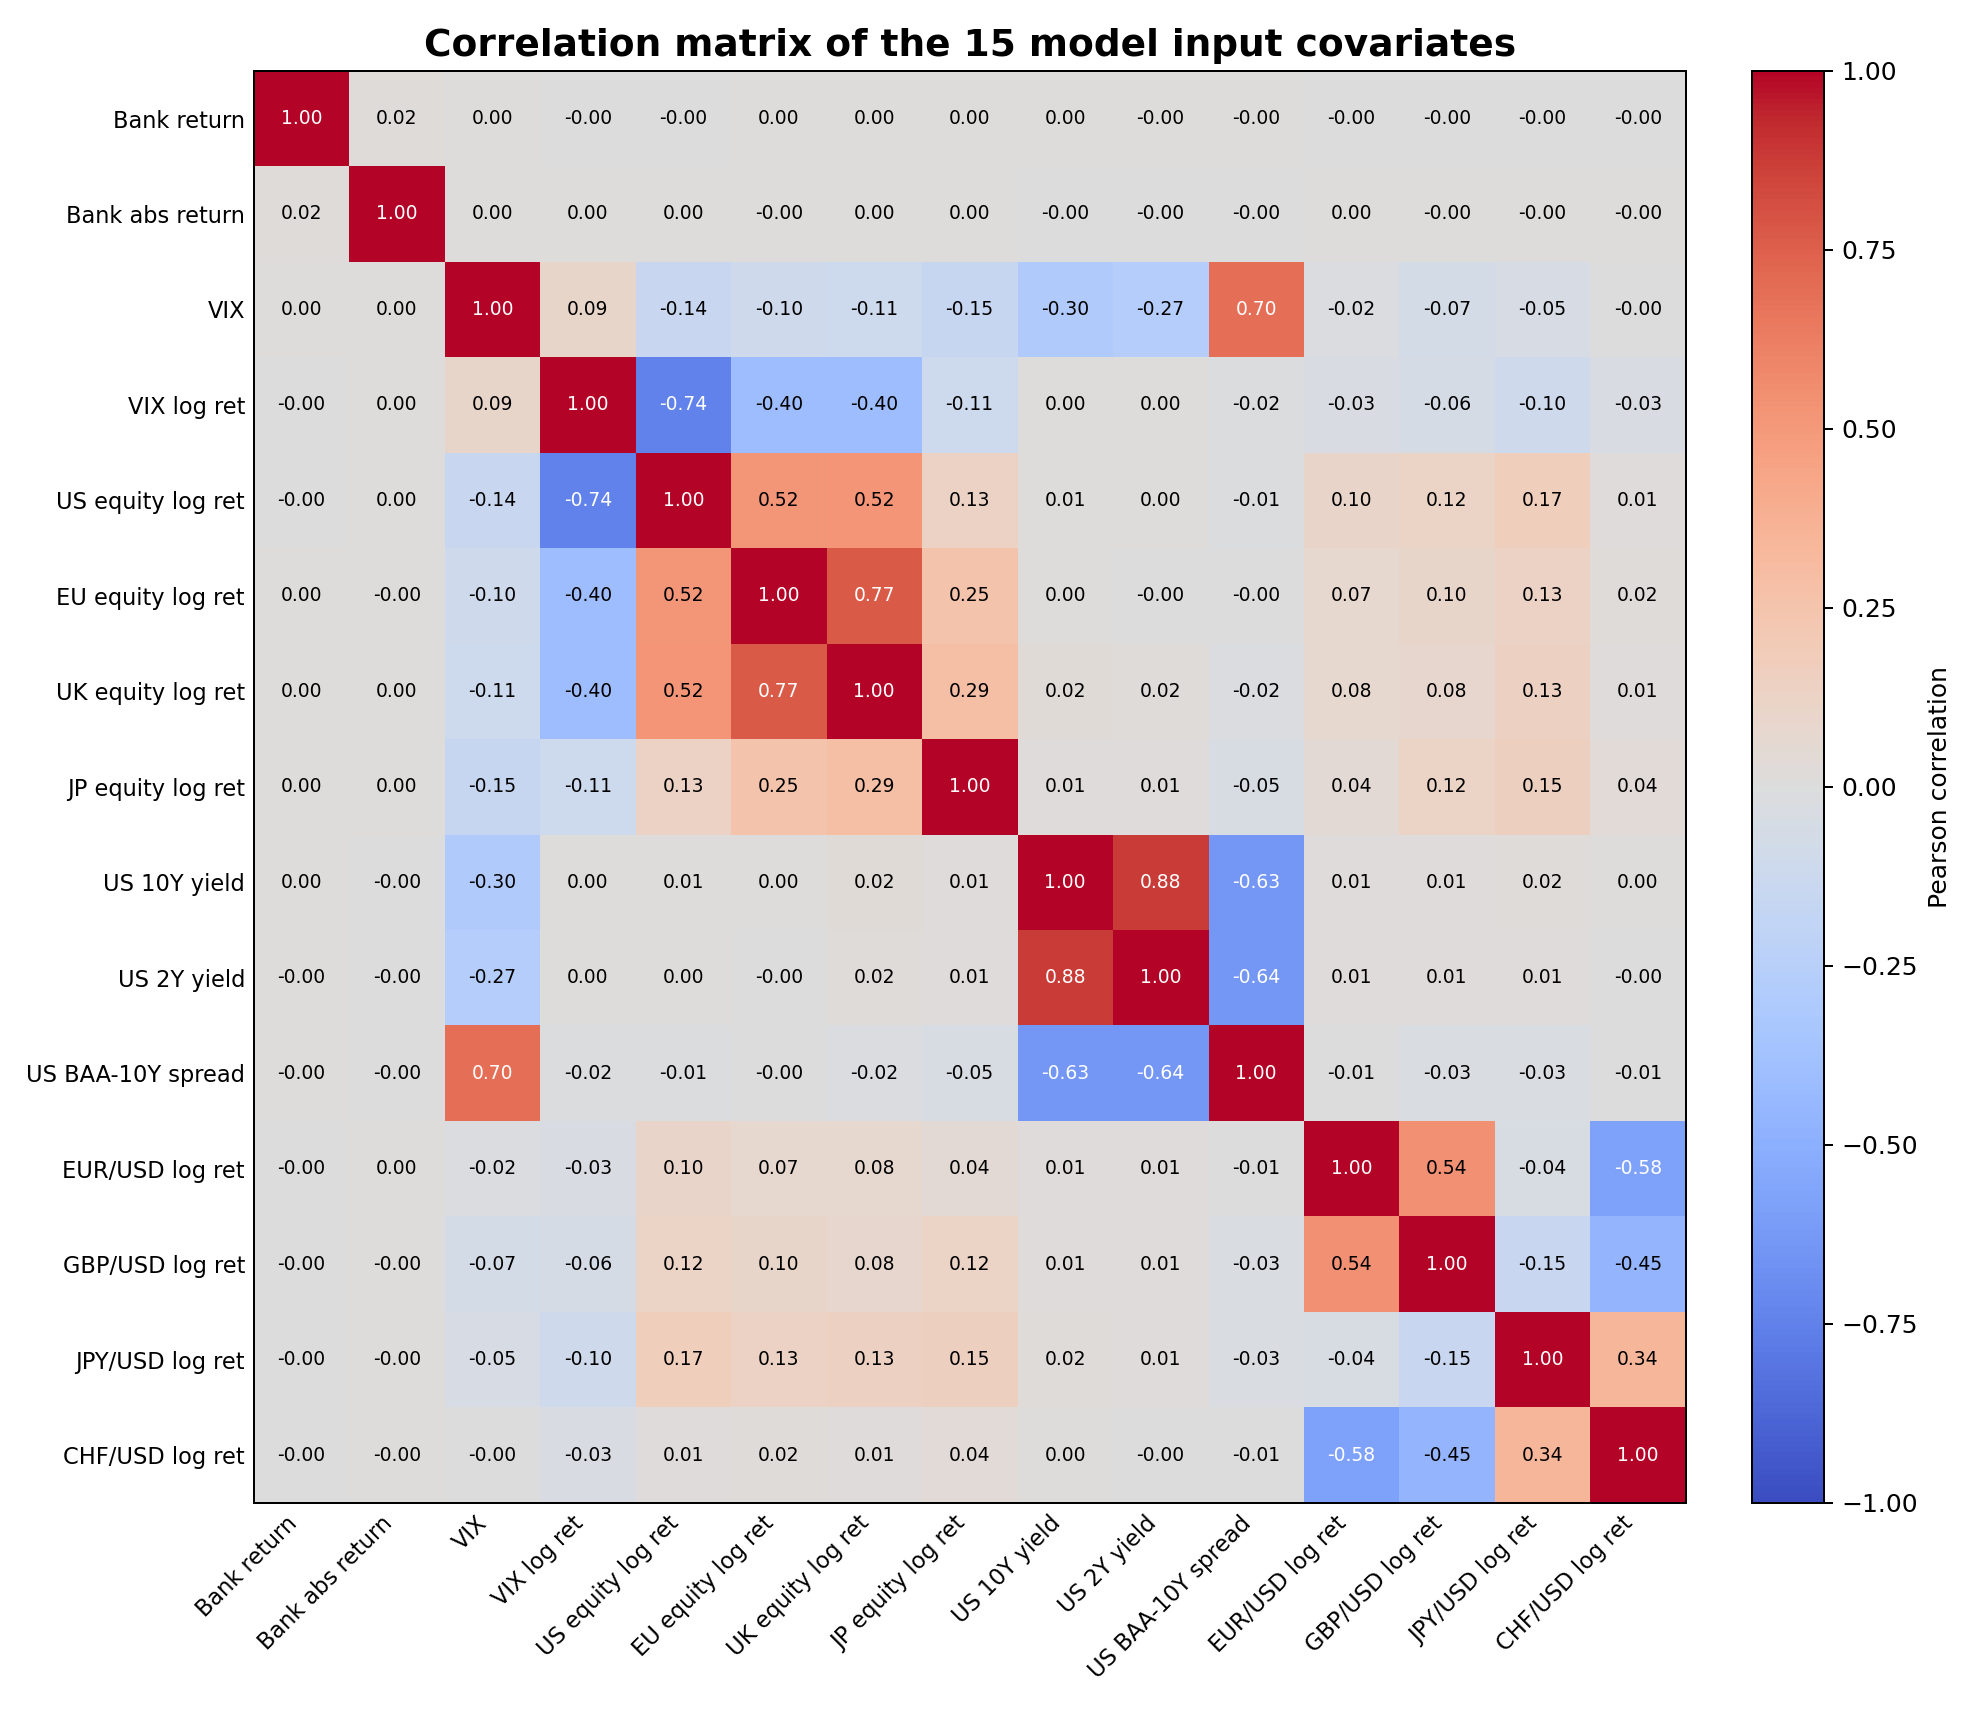
\includegraphics[width=\textwidth]{img/model_input_correlation_matrix.png}
%\captionof{figure}{Pearson correlation matrix for the 15 standardised covariates passed to the forecasting models.}
\end{minipage}
\end{minipage}

\section{Forecasting Loss}

For bank \(i\) on rebalance date \(t\), the response is the next-day USD log return \(y_{t+1,i}\). The information vector \(x_{t,i}\) contains only characteristics known by the date-\(t\) close. The linear benchmark solves ridge regression:

\[\hat\beta_\lambda=\arg\min_\beta \sum_{(t,i)\in\mathcal{D}_{train}}\left(y_{t+1,i}-\beta_0-x_{t,i}^\top\beta\right)^2+\lambda\lVert\beta\rVert_2^2,\]

with the intercept left unpenalised. The three specifications differ in how similarity between two standardised bank-date vectors is measured:

\[\begin{aligned}\kappa_{\mathrm{lin}}(x,x') &= x^\top x',\\\kappa_{\mathrm{poly}}(x,x') &= (c+x^\top x')^2,\\\kappa_{\mathrm{rbf}}(x,x') &= \exp\{-\gamma\lVert x-x'\rVert_2^2\}.\end{aligned}\]

Financially, the linear kernel is the low-variance benchmark for additive exposures to rates, spreads, FX and broad equity regimes. The degree-2 polynomial kernel is useful when pairwise interactions matter, for example when the effect of VIX depends on recent bank volatility or regional rate moves. The Gaussian/RBF kernel is a local-similarity model: it gives more weight to observations with nearby macro-financial states and is natural when crisis or calm regimes cluster in feature space, although it can overfit noisy daily returns.

All hyperparameters are selected before the active block is evaluated. Forecasting hyperparameters, including the ridge penalty \(\lambda\) and kernel-specific nonlinear parameters, are chosen on the validation window by point-forecast RMSE. The mean-variance covariance regularisation parameter \(\gamma\) is then selected economically: validation forecasts are used directly as expected returns in a constrained MVE problem with \(\widehat\Sigma+\gamma I\), and the selected value maximises daily certainty-equivalent utility, \( \bar R - A\sigma^2/2 \), with risk aversion \(A=3\).

\section{Rolling Calibration}

Each active block uses the previous 24 months: 18 months for training and 6 months for validation. The selected parameters are then fixed for the following 6 active months, giving a rolling train-validation-test design in which hyperparameters are chosen only from past data and never from the active evaluation period.

The experiment contains 42 independent semi-annual active blocks. They use the same deterministic data inputs but have separate fitted parameters, so they can be processed in parallel and then recombined in block/date order. The default desktop setup starts from 10 configurable workers.

The first active block starts on 2005-01-01, so the initial train-validation window begins around 2003-01-01 and the reported evaluation runs through the available 2025 observations. This roughly twenty-year window includes the 2008 global financial crisis, the 2011--2012 euro-area stress episode and the 2020 COVID shock, making the test period informative beyond calm-market conditions.

The semi-annual update frequency balances adaptiveness and computation: parameters can change through time, but the experiment remains auditable without requiring daily re-estimation and validation over many grid points.

\begin{figure}[H]\centering
\begin{minipage}[t]{0.315\textwidth}
\centering

\includegraphics[width=\linewidth]{img/parameter_evolution_lambda_linear.png}
\par\footnotesize Linear kernel constrained MVE
\end{minipage}
\hfill
\begin{minipage}[t]{0.315\textwidth}
\centering

\includegraphics[width=\linewidth]{img/parameter_evolution_lambda_polynomial.png}
\par\footnotesize Polynomial degree-2 kernel constrained MVE
\end{minipage}
\hfill
\begin{minipage}[t]{0.315\textwidth}
\centering

\includegraphics[width=\linewidth]{img/parameter_evolution_lambda_gaussian.png}
\par\footnotesize Gaussian RBF kernel constrained MVE
\end{minipage}
\caption{Semi-annual ridge penalties. Each panel shows one kernel at a time.}
\end{figure}

\begin{figure}[H]\centering
\begin{minipage}[t]{0.315\textwidth}
\centering

\includegraphics[width=\linewidth]{img/parameter_evolution_gamma_linear.png}
\par\footnotesize Linear kernel constrained MVE
\end{minipage}
\hfill
\begin{minipage}[t]{0.315\textwidth}
\centering

\includegraphics[width=\linewidth]{img/parameter_evolution_gamma_polynomial.png}
\par\footnotesize Polynomial degree-2 kernel constrained MVE
\end{minipage}
\hfill
\begin{minipage}[t]{0.315\textwidth}
\centering

\includegraphics[width=\linewidth]{img/parameter_evolution_gamma_gaussian.png}
\par\footnotesize Gaussian RBF kernel constrained MVE
\end{minipage}
\end{figure}

\begin{figure}[H]
\centering
\begin{minipage}[t]{0.42\textwidth}
\centering

\includegraphics[width=\textwidth]{img/parameter_evolution_coef0.png}
\end{minipage}
\hfill
\begin{minipage}[t]{0.56\textwidth}
\centering

\includegraphics[width=\textwidth]{img/parameter_evolution_gaussian_kernel_gamma.png}
\end{minipage}
\caption{Kernel-specific nonlinear calibration parameters.}
\end{figure}

\section{Portfolio Construction}

The active portfolio is implemented as a constrained regularised mean-variance allocation. On each active date, kernel forecasts are used directly as expected returns \(\widehat\mu_t\), while the covariance matrix \(\widehat\Sigma_t\) is estimated only from the training-window asset returns of the corresponding rolling block and regularised as \(\widehat\Sigma_t+\gamma I\). The optimisation is
\vspace{-0.125cm}
\[
\max_w\; \widehat\mu_t^\top w-\frac{A}{2}w^\top(\widehat\Sigma_t+\gamma I)w,
\quad
\sum_i w_i=1,
\quad
1\%\le w_i\le 7\%.
\vspace{-0.125cm}
\]

The regularisation parameter \(\gamma\) is selected on the validation window and fixed before the following six-month active block begins. Asset log returns are converted to simple returns for portfolio aggregation and then converted back to portfolio log returns for compounding statistics.

The 1\%--7\% box constraints make the kernel portfolios economically comparable to the equal-weight benchmark and prevent unstable daily reallocations. Without constraints, small forecast differences could lead to excessive concentration in a few banks, institutions or regions. The lower bound keeps every selected bank represented, while the upper bound limits single-name and regional exposure. The portfolio therefore remains a genuine mean-variance allocation driven by kernel forecasts and the estimated covariance matrix, but within a controlled diversified risk space where models can still improve performance through better tilts, lower drawdowns, higher Sharpe ratios or stronger cumulative returns.

The strategy is kept long-only because short positions would require additional assumptions on margin requirements, leverage limits, borrow availability, stock-loan interest, short-sale costs and transaction costs. This makes the implementation simpler and more defensible: forecasts can tilt the portfolio, but cannot introduce unmodelled financing or borrowing effects.

\section{Rolling Out-of-Sample Results}
\vspace{-0.25cm}
\begin{table}[H]\centering
\begingroup\footnotesize
\setlength{\tabcolsep}{3.2pt}
\begin{tabular}{lrrrrrr}
\toprule
Strategy & Mean log & Vol log & Total log & Sharpe & Cum. ret. & Max DD \\
\midrule
Equal weight & 0.000266 & 0.017985 & 1.4558 & 0.235 & 3.288 & -78.7\% \\
Linear kernel constrained MVE & 0.000842 & 0.015472 & 4.6126 & 0.864 & 99.741 & -57.6\% \\
Polynomial degree-2 kernel constrained MVE & 0.000714 & 0.015486 & 3.9115 & 0.732 & 48.972 & -60.8\% \\
Gaussian RBF kernel constrained MVE & 0.000666 & 0.015726 & 3.6455 & 0.672 & 37.300 & -59.3\% \\
\bottomrule
\end{tabular}
%\caption{Comparative statistics computed on the common evaluation period across all strategies.}
\endgroup
\end{table}

In the current run, Linear kernel constrained MVE is the strongest portfolio by annualised Sharpe (0.864). Annualised Sharpe ratios are: Equal weight 0.235; Linear kernel constrained MVE 0.864; Polynomial degree-2 kernel constrained MVE 0.732; Gaussian RBF kernel constrained MVE 0.672. The cumulative-return gap is large because small daily log-return differences compound over the full out-of-sample sample.

\begin{figure}[H]\centering

\includegraphics[width=0.90\textwidth]{img/cumulative_returns_linear_vs_equal_weight.png}
\vspace{0.45em}

\includegraphics[width=0.90\textwidth]{img/cumulative_returns_polynomial_vs_equal_weight.png}
\vspace{0.45em}

\includegraphics[width=0.90\textwidth]{img/cumulative_returns_gaussian_vs_equal_weight.png}
\vspace{0.45em}
\end{figure}
\begin{figure}[H]\centering

\includegraphics[width=0.90\textwidth]{img/cumulative_returns_all_kernels.png}
\caption{Cumulative performance split into four vertical panels: three kernel-vs-equal-weight comparisons followed by one combined panel with all kernels and the benchmark.}
\end{figure}


\section{Risk Diagnostics}

Using paired daily drawdown differences with a Newey--West correction, all three kernel portfolios have significantly less severe drawdowns than equal weight (smallest comparison p=$1.1\times 10^{-28}$). Their maximum drawdowns are Linear kernel constrained MVE (-57.6\%), Polynomial degree-2 kernel constrained MVE (-60.8\%), Gaussian RBF kernel constrained MVE (-59.3\%), versus -78.7\% for equal weight. Within the active kernels, Linear kernel also has a statistically less severe drawdown path than the nonlinear kernels (best p=$2.9\times 10^{-8}$), although the economic gap among kernel drawdowns is much smaller than the gap versus equal weight.

\begin{figure}[H]\centering

\includegraphics[width=0.90\textwidth]{img/drawdown_linear_vs_equal_weight.png}
\vspace{0.45em}

\includegraphics[width=0.90\textwidth]{img/drawdown_polynomial_vs_equal_weight.png}
\vspace{0.45em}

\includegraphics[width=0.90\textwidth]{img/drawdown_gaussian_vs_equal_weight.png}
\vspace{0.45em}

\includegraphics[width=0.90\textwidth]{img/drawdown_all_kernels.png}
\caption{Drawdown comparison split into four vertical panels: three kernel-vs-equal-weight comparisons followed by one combined panel with all kernels and the benchmark.}
\end{figure}

The rolling-return and rolling-volatility diagnostics are still generated in the repository outputs. In words, the active kernels separate mainly through rolling returns and drawdown control rather than through a large volatility gap: the final daily volatility is lower for all active kernels than for equal weight, while their rolling volatilities remain close to one another through most of the sample.

\begin{figure}[H]\centering

\includegraphics[width=0.96\textwidth]{img/rolling_sharpe.png}
\caption{Rolling 252-day annualized Sharpe ratio.}
\end{figure}

The crisis plots matter because the universe is a long-only bank-sector universe. in 2008 global financial crisis, Linear kernel constrained MVE has the best window return (9.1\%), while the deepest drawdown is -75.2\%; in 2012 euro stress, Polynomial degree-2 kernel constrained MVE has the best window return (71.2\%), while the deepest drawdown is -40.3\%; in 2020 covid shock, Linear kernel constrained MVE has the best window return (2.6\%), while the deepest drawdown is -46.7\%. The models reduce some crisis losses relative to equal weight in this run, but they do not eliminate common banking-sector risk.

\begin{figure}[H]\centering

\includegraphics[width=0.9\textwidth]{img/crisis_2008_global_financial_crisis.png}
\vspace{0.45em}

\includegraphics[width=0.9\textwidth]{img/crisis_2012_euro_stress.png}
\vspace{0.45em}

\includegraphics[width=0.9\textwidth]{img/crisis_2020_covid_shock.png}
\caption{Performance during the predefined crisis windows.}
\end{figure}

\section{Geographic Exposure and Weights}

Each stacked panel aggregates daily bank weights by region, so each band is the portfolio share allocated to that geography. The palette is fixed in the order US, UK, EU, CH and JP. The paired Newey--West exposure tests compare each kernel's daily regional weight with the equal-weight regional exposure. The strongest persistent tilts are: Linear kernel constrained MVE overweights JP by 1.84 pp (p=$3.3\times 10^{-73}$) and underweights EU by 3.31 pp (p=$8.3\times 10^{-39}$); Polynomial degree-2 kernel constrained MVE overweights JP by 1.17 pp (p=$1.1\times 10^{-35}$) and underweights EU by 1.58 pp (p=$2.1\times 10^{-14}$); Gaussian RBF kernel constrained MVE overweights JP by 1.58 pp (p=$1.6\times 10^{-57}$) and underweights EU by 2.33 pp (p=$5.1\times 10^{-24}$).


\vspace{-0.125cm}

\begin{figure}[H]\centering

\includegraphics[width=0.9\textwidth]{img/geographic_exposure.png}
\caption{Daily geographic exposure of the final portfolios, with region legend above the panels.}
\vspace{-0.125cm}
\end{figure}

The weight heatmaps use a colour scale focused on the active 1\%-7\% range. This makes it easier to see which names are near the lower bound, near the upper bound, or close to the equal-weight allocation. Feasibility checks in the code enforce full investment and the 1\%--7\% box within numerical tolerance for the constrained MVE portfolios.

The heatmaps also show how often the constrained MVE optimizer uses the box limits. Using a narrow 0.05 percentage-point tolerance around the 1\% and 7\% limits, Gaussian RBF kernel constrained MVE pushes weights to a bound most often (74.8\% of asset-date observations), while Polynomial degree-2 kernel constrained MVE is the least bound-driven (65.1\%). Looking instead at weights within one percentage point of the roughly 4\% equal-weight allocation, Polynomial degree-2 kernel constrained MVE is closest to equal weight most often (15.5\%). So the active portfolios are not constantly pinned to the limits: a large share of positions remains near the benchmark allocation, while nonlinear kernels can still create stronger mean-variance tilts than the linear benchmark.

\begin{figure}[H]\centering
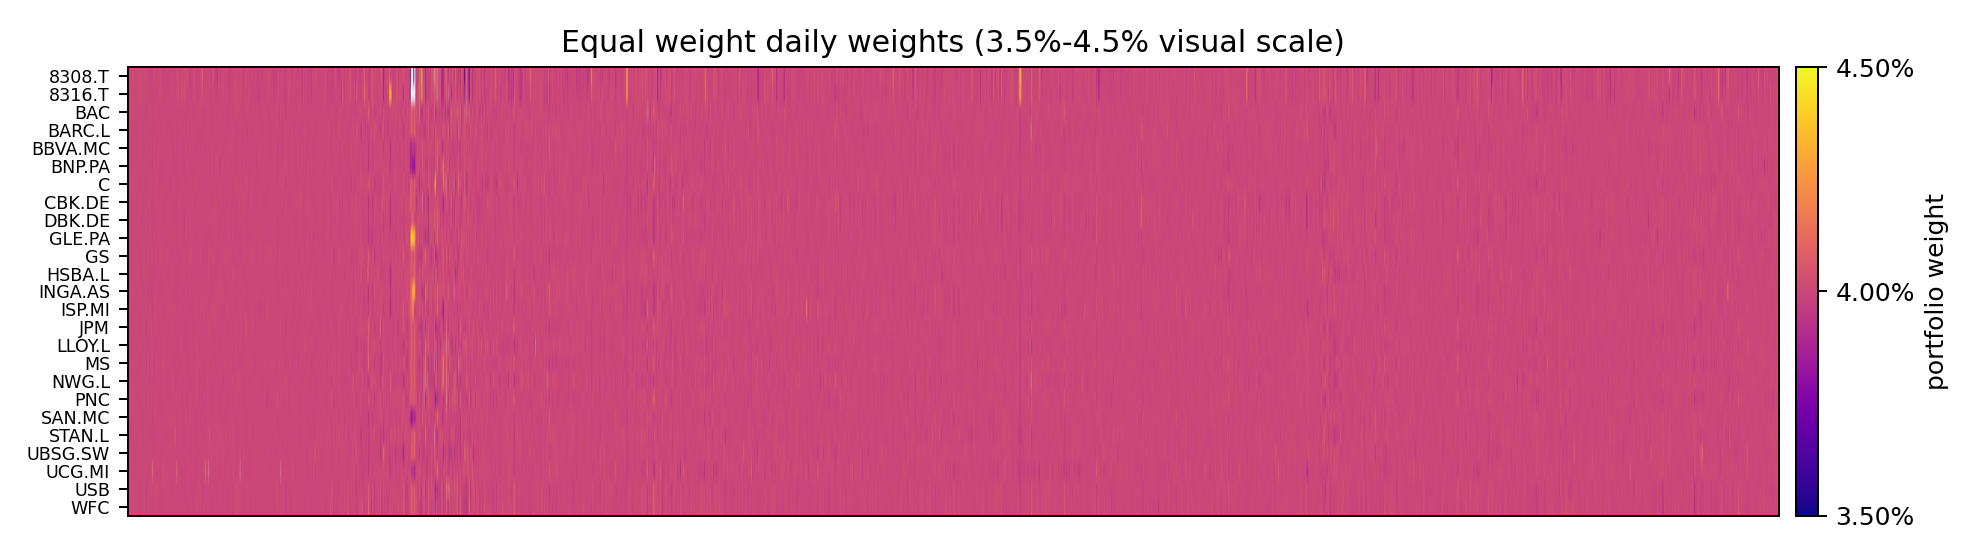
\includegraphics[width=0.9\textwidth]{img/weight_dynamics_equal_weight.png}
\end{figure}
\begin{figure}[H]\centering
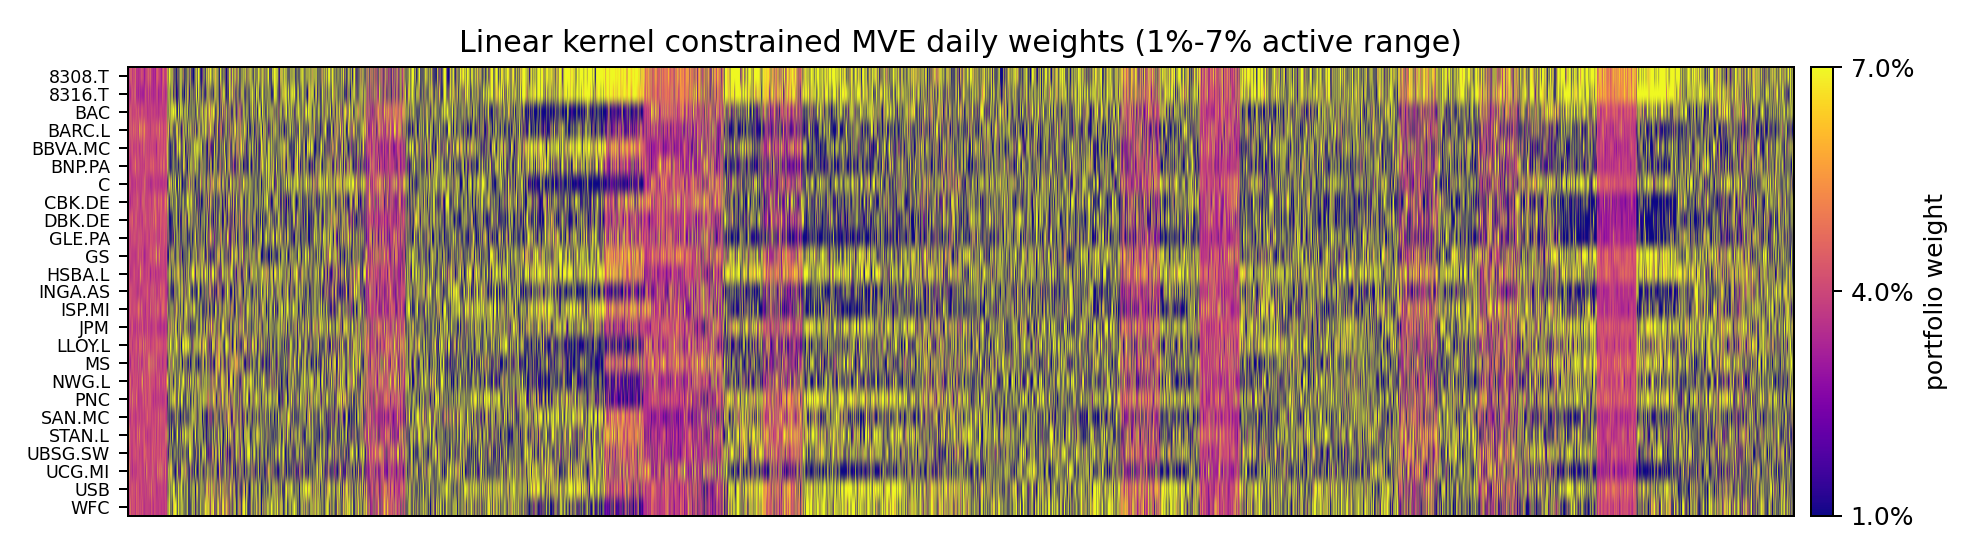
\includegraphics[width=0.9\textwidth]{img/weight_dynamics_linear.png}

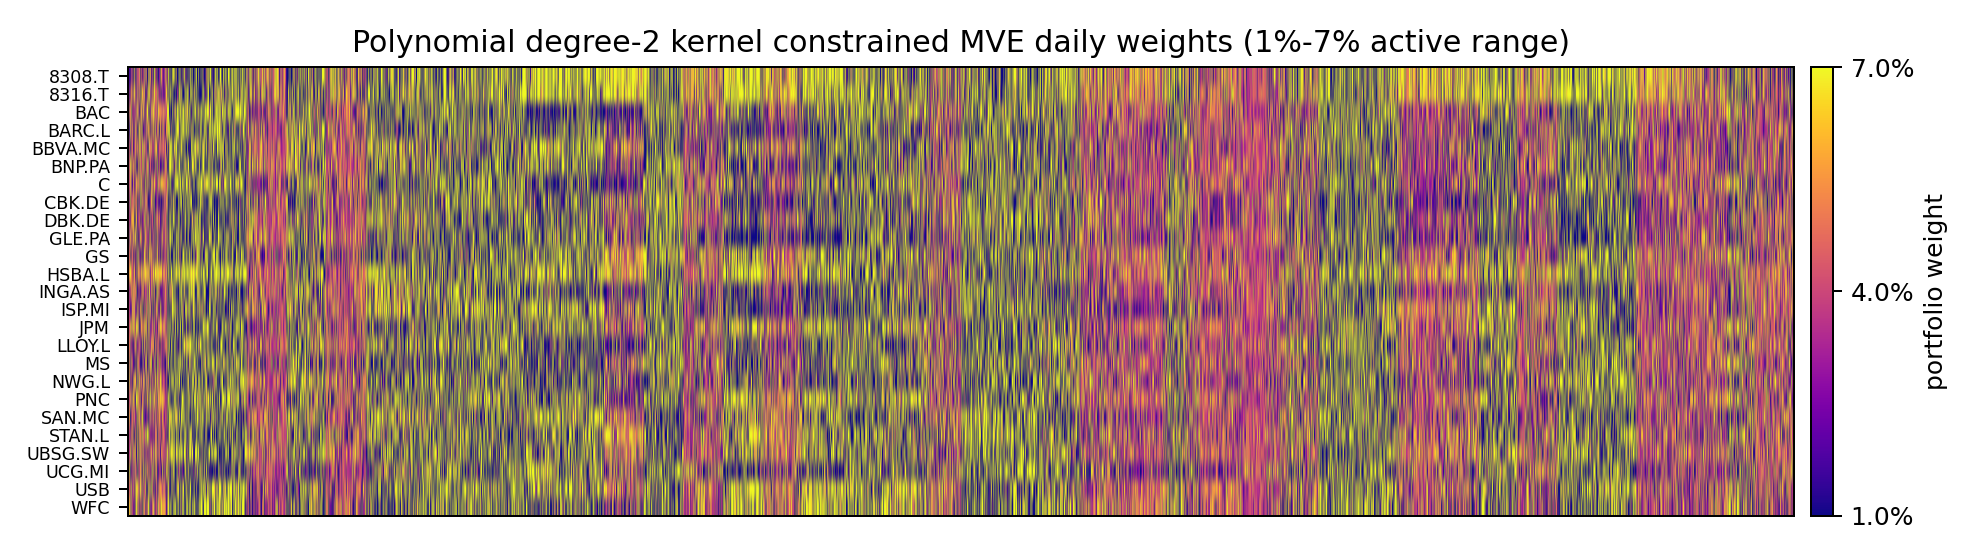
\includegraphics[width=0.9\textwidth]{img/weight_dynamics_polynomial.png}

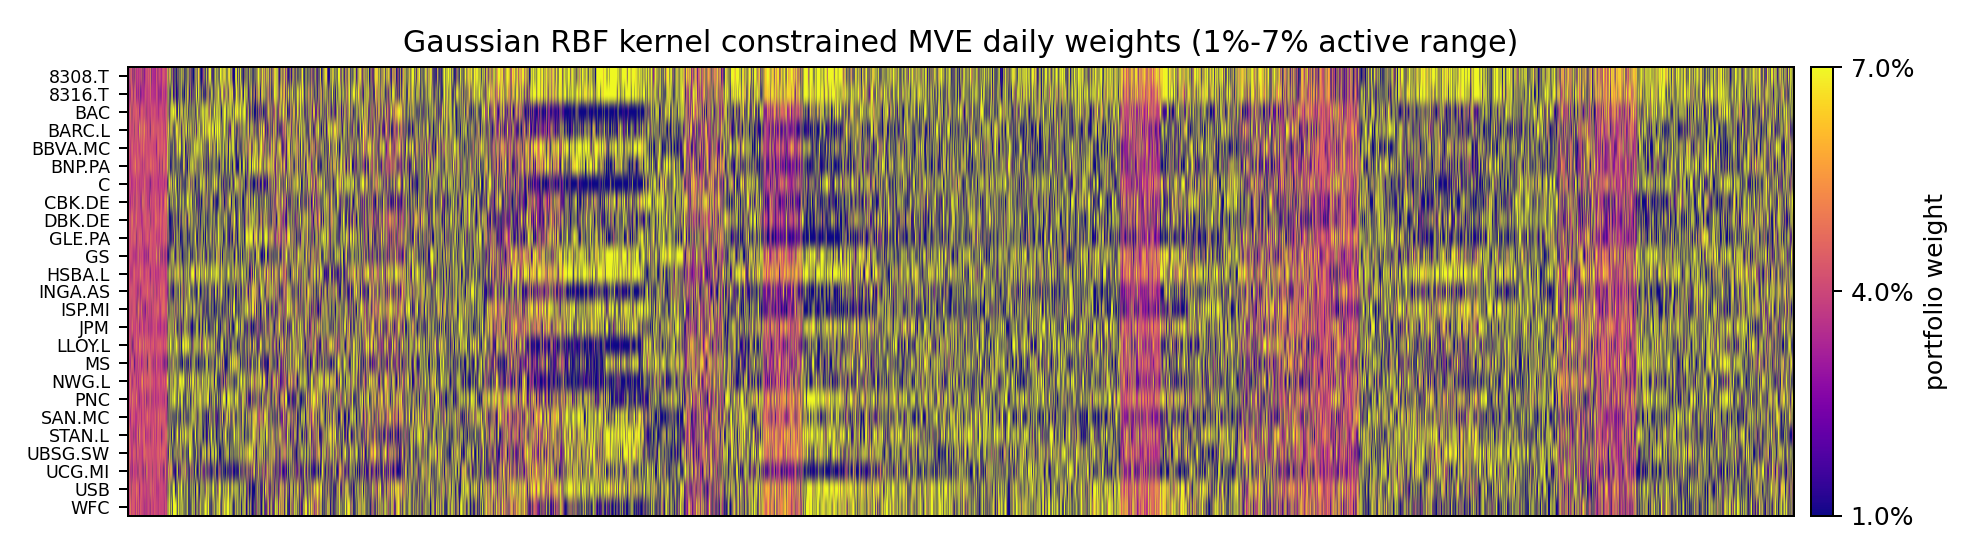
\includegraphics[width=0.9\textwidth]{img/weight_dynamics_gaussian.png}
\caption{Daily asset weights and weight-sum controls.}
\vspace{-0.125cm}
\end{figure}

\section{Forecast Diagnostics}
\vspace{-0.125cm}
The active forecast diagnostics are separated from portfolio performance. Daily bank returns are difficult to predict in squared-error terms, so the table evaluates point forecasts, while the portfolio results assess whether noisy signals can still generate useful covariance-aware tilts. In this run, Linear kernel constrained MVE and Gaussian RBF kernel constrained MVE remain closest to the mean-return benchmark, whereas Polynomial degree-2 kernel constrained MVE performs much worse as a point forecast.

For block-level OOS \(R^2\), zero corresponds to the squared-error performance of the mean-return benchmark. Positive values indicate meaningful out-of-sample explanatory power, while strongly negative values mean that forecast errors are much larger than benchmark errors. The three-column figure reports separate per-kernel panels over the full rolling-block series. Linear kernel constrained MVE ranges from a peak of 0.051 on 2008-01-01 to a trough of -0.192 on 2016-07-01; Polynomial degree-2 kernel constrained MVE ranges from -0.034 on 2006-01-02 to -14.513 on 2015-01-01; Gaussian RBF kernel constrained MVE ranges from 0.043 on 2013-01-01 to -0.166 on 2022-07-01. Overall, the linear and Gaussian panels stay much closer to zero, while the polynomial panel shows the deepest negative episodes.

\begin{figure}[H]\centering
\begin{minipage}[t]{0.315\textwidth}
\centering

\includegraphics[width=\linewidth]{img/oos_r2_linear_compact.png}
\par\footnotesize\textbf{Linear kernel}
\end{minipage}
\hfill
\begin{minipage}[t]{0.315\textwidth}
\centering

\includegraphics[width=\linewidth]{img/oos_r2_polynomial_compact.png}
\par\footnotesize\textbf{Polynomial degree-2 kernel}
\end{minipage}
\hfill
\begin{minipage}[t]{0.315\textwidth}
\centering

\includegraphics[width=\linewidth]{img/oos_r2_gaussian_compact.png}
\par\footnotesize\textbf{Gaussian RBF kernel}
\end{minipage}
\caption{Block-level out-of-sample forecast $R^2$ by kernel. Each panel is generated as a separate compact image and arranged in a three-column row; the x-axis spans the full active rolling-block series without dropping observations.}
\end{figure}

\begin{table}[H]\centering\small
\begin{tabular}{lrrrrr}
\toprule
Model & OOS $R^2$ & RMSE & MAE & Bias & Obs. \\
\midrule
Linear kernel constrained MVE & -0.0239 & 0.0226 & 0.0135 & -0.000342 & 136900 \\
Polynomial degree-2 kernel constrained MVE & -1.5134 & 0.0354 & 0.0184 & -0.001141 & 136900 \\
Gaussian RBF kernel constrained MVE & -0.0291 & 0.0226 & 0.0134 & 0.000058 & 136900 \\
\bottomrule
\end{tabular}
\caption{Forecast diagnostics on the active out-of-sample blocks.}
\end{table}

Table 2 is a point-forecast table, not a portfolio-performance table. An OOS \(R^2\) close to zero means that the model is roughly tying the simple mean-return benchmark in squared-error terms; a large negative value means that point forecasts are materially worse than that benchmark. In this run, Linear kernel constrained MVE and Gaussian RBF kernel constrained MVE stay closest to zero, and Linear kernel constrained MVE has the lowest RMSE while Gaussian RBF kernel constrained MVE has the lowest MAE. The weakest point-forecast specification is Polynomial degree-2 kernel constrained MVE, which is furthest from zero. The daily biases are small relative to the RMSEs, so the main issue is not a simple constant offset; it is unstable expected-return noise and very large forecast errors in some blocks.

\begin{figure}[H]\centering
\begin{minipage}[t]{0.315\textwidth}
\centering

\includegraphics[width=\linewidth]{img/prediction_error_scatter_linear.png}
\par\footnotesize Linear kernel constrained MVE
\end{minipage}
\hfill
\begin{minipage}[t]{0.315\textwidth}
\centering

\includegraphics[width=\linewidth]{img/prediction_error_scatter_polynomial.png}
\par\footnotesize Polynomial degree-2 kernel constrained MVE
\end{minipage}
\hfill
\begin{minipage}[t]{0.315\textwidth}
\centering

\includegraphics[width=\linewidth]{img/prediction_error_scatter_gaussian.png}
\par\footnotesize Gaussian RBF kernel constrained MVE
\end{minipage}
\caption{Forecast residuals against predicted returns for the three kernel specifications, shown on common axes.}
\end{figure}

\begin{figure}[H]\centering
\begin{minipage}[t]{0.315\textwidth}
\centering

\includegraphics[width=\linewidth]{img/prediction_error_distribution_linear.png}
\par\footnotesize Linear kernel constrained MVE
\end{minipage}
\hfill
\begin{minipage}[t]{0.315\textwidth}
\centering

\includegraphics[width=\linewidth]{img/prediction_error_distribution_polynomial.png}
\par\footnotesize Polynomial degree-2 kernel constrained MVE
\end{minipage}
\hfill
\begin{minipage}[t]{0.315\textwidth}
\centering

\includegraphics[width=\linewidth]{img/prediction_error_distribution_gaussian.png}
\par\footnotesize Gaussian RBF kernel constrained MVE
\end{minipage}
\caption{Out-of-sample forecast-error distributions by kernel, shown on a common horizontal and vertical scale.}
\end{figure}

\begin{table}[H]\centering\small
\begin{tabular}{lrrrrr}
\toprule
Model & JB p-value & Skewness & Excess kurt. & Outlier 3$\sigma$ & Tail ratio \\
\midrule
Linear kernel constrained MVE & 0.00e+00 & -0.691 & 26.89 & 1.73\% & 6.4x \\
Polynomial degree-2 kernel constrained MVE & 0.00e+00 & -4.212 & 111.17 & 1.42\% & 5.3x \\
Gaussian RBF kernel constrained MVE & 0.00e+00 & -0.623 & 27.65 & 1.71\% & 6.3x \\
\bottomrule
\end{tabular}
\caption{Normality and tail diagnostics for out-of-sample forecast errors. Jarque--Bera tests normality through skewness and kurtosis; outliers are errors more than three empirical standard deviations from the model mean error.}
\end{table}

The normality check confirms that forecast errors are not Gaussian. All reported JB p-values are effectively zero: under the null hypothesis of Gaussian forecast errors, the probability of observing skewness and kurtosis this extreme is numerically negligible. The normality null is therefore rejected for every kernel. The tail ratio is the empirical share of errors more than three standard deviations from the model mean divided by the normal-theory benchmark of about 0.27\%. Here the ratios range from 5.3x to 6.4x, so extreme misses are several times more frequent than a Gaussian error model would imply. The 3-sigma outlier shares are all around 1.4\%--1.7\%, far above the Gaussian benchmark. All excess-kurtosis values are positive, which means the distributions are fat-tailed rather than bell-shaped; Polynomial degree-2 kernel constrained MVE is the most extreme case. This is financially important: in bank equities, the largest errors tend to occur around stress, policy surprises and broad risk-on/risk-off repricing, exactly when a portfolio rule is most sensitive to ranking errors.


\section{Optimality Summary}

As a diagnostic extension, the maximum asset-weight cap is searched on a grid from 4.0\% to 20.0\% in 0.1 percentage-point steps, while keeping the minimum weight fixed at 1\%. For each kernel, the selected cap is reported under three portfolio-level objectives: annualised Sharpe, cumulative return and maximum drawdown.

\begin{table}[H]\centering\scriptsize
\resizebox{\textwidth}{!}{%
\begin{tabular}{lllrrrr}
\toprule
Objective & Kernel & Best interval & Sharpe & Cum. return & Max DD & Daily vol. \\
\midrule
Max Sharpe & Linear kernel constrained MVE & 1.0\%-12.8\% & 0.967 & 221.32 & -58.5\% & 0.0162 \\
Max Sharpe & Polynomial degree-2 kernel constrained MVE & 1.0\%-13.5\% & 0.814 & 94.74 & -59.5\% & 0.0162 \\
Max Sharpe & Gaussian RBF kernel constrained MVE & 1.0\%-15.1\% & 0.723 & 59.42 & -60.0\% & 0.0164 \\
Max cumulative return & Linear kernel constrained MVE & 1.0\%-18.7\% & 0.960 & 251.65 & -60.4\% & 0.0167 \\
Max cumulative return & Polynomial degree-2 kernel constrained MVE & 1.0\%-16.3\% & 0.804 & 96.46 & -60.5\% & 0.0165 \\
Max cumulative return & Gaussian RBF kernel constrained MVE & 1.0\%-16.0\% & 0.722 & 59.75 & -60.7\% & 0.0165 \\
Min max drawdown & Linear kernel constrained MVE & 1.0\%-5.7\% & 0.777 & 60.62 & -56.0\% & 0.0154 \\
Min max drawdown & Polynomial degree-2 kernel constrained MVE & 1.0\%-5.4\% & 0.668 & 33.78 & -58.1\% & 0.0154 \\
Min max drawdown & Gaussian RBF kernel constrained MVE & 1.0\%-5.4\% & 0.639 & 29.51 & -58.3\% & 0.0155 \\
\bottomrule
\end{tabular}
}
\caption{Best maximum-weight cap by kernel and portfolio-level objective. The lower bound remains 1\%; only the upper cap is selected on the grid.}
\end{table}

The fixed 1\%--7\% box used in the main report is not the ex-post optimum in this cap grid: Sharpe and cumulative-return objectives choose looser caps above 7\%, while the max-drawdown objective chooses tighter caps around 5.4\%--5.7\%. This does not invalidate the main specification, because the 1\%--7\% rule is an ex-ante diversification constraint rather than a realised-metric optimum.

These are allocation-level results only. The rolling forecasts, forecast errors and OOS \(R^2\) are unchanged by the cap search, so the cap that is optimal for Sharpe, cumulative return or drawdown is not necessarily optimal for prediction accuracy. Relative to the fixed 1\%--7\% portfolios, 3 of the 9 selected rows have both lower daily volatility and a less severe maximum drawdown, 5 of 9 have a less severe maximum drawdown, and 6 of 9 have higher or equal daily volatility. Thus, the max-drawdown-selected rows are the stability-improving cases, while the Sharpe- and cumulative-return-selected rows mainly improve return metrics by allowing looser caps.


\section{Conclusion}

This project shows that daily macro-financial signals can add portfolio value in a global bank universe, even though next-day return prediction remains noisy. The forecast diagnostics do not support a strong predictability claim: out-of-sample \(R^2\) values are weak or negative, and forecast errors are fat-tailed. The relevant result is instead portfolio-level: constrained, covariance-aware mean-variance tilts can improve risk-adjusted performance relative to equal weight.

In this run, the linear kernel constrained MVE is the strongest and most stable active specification. Its advantage suggests that most useful information is low-dimensional and regime-based: rates, spreads, FX variables and regional equity indices already capture broad monetary-policy, funding-stress and risk-cycle movements. The polynomial and Gaussian kernels add nonlinear flexibility, but on next-day equity returns this flexibility can also amplify noise.

The fixed 1\%--7\% weight box should be interpreted as an ex-ante diversification rule, not as an ex-post optimum. The cap-search extension shows that looser caps can improve return-based metrics, while tighter caps can improve drawdown stability. This confirms that allocation constraints matter, but it does not change the forecast comparison because the predictions are unchanged.

The main limitations are practical. Transaction costs, bid-ask spreads, taxes, funding costs and market impact are not deducted. The bank universe may suffer from survivorship bias because it is selected using data availability. Adjusted close prices include dividend and split adjustments, but realised after-tax returns can differ. Since the strategy is long-only and sector-specific, it can reduce but not eliminate common banking-crisis risk.

Future extensions should add realistic trading frictions, turnover penalties, transaction-cost-aware rebalancing and a more formal treatment of delisted or failed banks. Broader hyperparameter grids, alternative rebalance horizons and daily recalibration could also be tested, provided that the same chronological validation discipline is preserved.

Overall, rolling kernel methods can add value in this constrained global-bank experiment, especially through the linear kernel, but the contribution is not precise return forecasting. It is a disciplined framework for turning weak daily macro-financial signals into diversified, no-look-ahead portfolio tilts.

\begingroup\raggedright

\begin{thebibliography}{9}

\bibitem{markowitz1952} Markowitz, H. (1952). Portfolio Selection. \textit{Journal of Finance}, 7(1), 77--91.

\bibitem{demiguel2009} DeMiguel, V., Garlappi, L., and Uppal, R. (2009). Optimal versus naive diversification. \textit{Review of Financial Studies}, 22(5), 1915--1953.

\bibitem{welchgoyal2008} Welch, I., and Goyal, A. (2008). A comprehensive look at the empirical performance of equity premium prediction. \textit{Review of Financial Studies}, 21(4), 1455--1531.

\bibitem{jagannathan2003} Jagannathan, R., and Ma, T. (2003). Risk reduction in large portfolios: why imposing the wrong constraints helps. \textit{Journal of Finance}, 58(4), 1651--1684.

\bibitem{githubrepo} F. Florio, P. Meloni, S. Messina, A. Sisto, and M. Zavatteri, \emph{Cross-Sectional Return Prediction for Global Banks with Rolling Kernel Calibration: supporting code}, GitHub repository, \url{https://github.com/SalvatoreMessina11/Kernel-Project.git}, accessed 17/05/2026.

\end{thebibliography}

\endgroup
\end{document}
